\documentclass[glossy,aspectratio=169]{beamer}
\beamertemplatenavigationsymbolsempty
\usepackage[utf8]{inputenc}
\useoutertheme{wuerzburg}
\useinnertheme[realshadow,corners=2pt,padding=2pt]{chamfered}
\usecolortheme{whale}
\usepackage[ngerman]{babel}
\usepackage{graphics, graphicx}
\usepackage{color}
\usepackage{latexsym}
\usepackage{etoolbox}
\usepackage{subfig}
\usepackage{tikz}
\PassOptionsToPackage{hyphens}{url}
\usepackage{hyperref}
\usepackage{url}
\usepackage{qrcode}
\usepackage{eurosym}

% Override these to reproduce a build, if you run
% "nix-build --argstr date YYYY-MM-DD" you don't need to change them manually:
\year=\year
\month=\month
\day=\day

\newcommand<>{\hover}[1]{\uncover#2{%
		\begin{tikzpicture}[remember picture,overlay]%
		\draw[fill,opacity=0.4] (current page.south west)
		rectangle (current page.north east);
		\node at (current page.center) {#1};
		\end{tikzpicture}}
}

\definecolor{pblue}{rgb}{0.13,0.13,1}
\definecolor{pgreen}{rgb}{0,0.5,0}
\definecolor{pred}{rgb}{0.9,0,0}
\definecolor{pgrey}{rgb}{0.46,0.45,0.48}
\definecolor{darkgreen}{rgb}{0,0.5,0}


\title{Fachschaftsvorstellung}
\author{\textbf{fsi}}

\begin{document}
	%\maketitle
	\begin{frame}
		\centering
		\includegraphics[width=0.8\textwidth]{pictures/fsilogo_neu.pdf}\\
		\vspace*{1cm}
		\begin{huge}
			Fachschaft? Kann man das essen?
		\end{huge}
	\end{frame}
	
	\begin{frame}{Wer sind wir?}
		\begin{figure}
			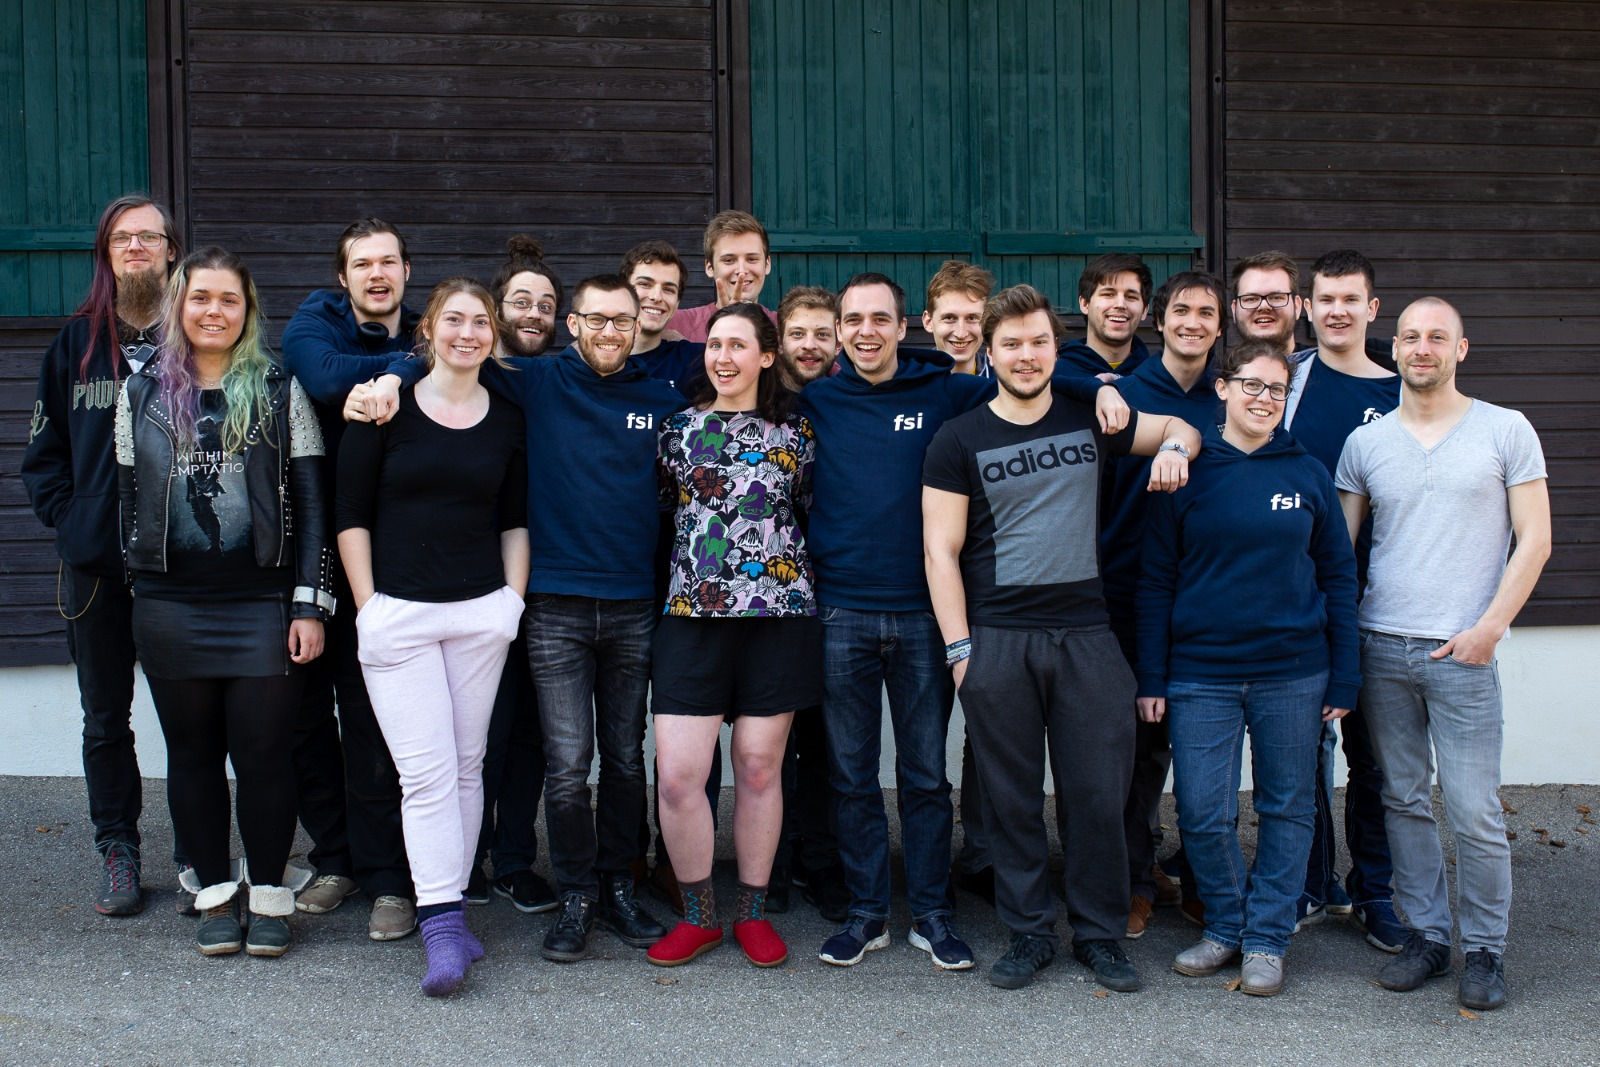
\includegraphics[height=0.9\textheight]{pictures/Gruppe19.jpeg}
		\end{figure}
	\end{frame}
	
 	
	\begin{frame}{Was machen wir?}
		\pause 
		\begin{itemize}[<+->]
			\item stehen in engem Kontakt mit der Professorenschaft
			\item können Probleme daher gut ansprechen
			\item (und meistens auch beheben)
			\item monatliche Treffen mit dem Fachbereich, um Problemen vorzubeugen
			\item[$\Rightarrow$] Wir brauchen euren Input!\\Also kommt zu uns, wenn ihr Probleme habt!
		\end{itemize}
	\end{frame}
	
	\begin{frame}{Studienberatung}
		\pause 
		\begin{itemize}[<+->]		
			\item \textbf{Informatik \& Bioinformatik}\quad Berater: Thomas Sachs\\
			E-Mail: studienberatung[@]informatik.uni-tuebingen.de
			
			\item \textbf{Kognitionswissenschaft}\quad 
			Berater: Paul Fischer \& Lia Schmid\\
			E-Mail: kogni-beratung[@]fsi.uni-tuebingen.de
			
			\item \textbf{Medieninformatik}\quad 
			Beraterin: Vanessa Kirchner\\
			E-Mail: medieninformatik[@]uni-tuebingen.de\\
			
			\item \textbf{Medizininformatik}\quad 		
			Berater: Felix Sieghörtner\\
			E-Mail: medizininformatik[@]uni-tuebingen.de
			
			\item \textbf{Lehramt}\quad 
			Beraterin: Saskia Honeck\\
			E-Mail: lehramt[@]informatik.uni-tuebingen.de
		\end{itemize}
	\end{frame}

	\begin{frame}{Server \& Administration}
		\pause 
		\begin{itemize}[<+->]			
			\item Betreiben und Warten von verschiedener Infrastruktur
			\begin{itemize}[<+->]
				\item Mailinglisten
				\item Prüfungsprotokolle-Interface (PPI)
				\item Abschlussarbeiten-Interface (AAI)
			\end{itemize}
		\end{itemize}
	\end{frame}
	
	\begin{frame}{Server \& Administration}
	\framesubtitle{Mailinglisten}
	\pause 
		\begin{columns}
			\begin{column}{.5\textwidth}
				\textbf{*-InformatikerInnen:}
				\small
				\begin{itemize}[<+->]
					\item \textbf{info-studium} 
					\item info-talk
					\item info-jobs
					\item sport
					\item coding
				\end{itemize}
			\end{column}
			\begin{column}{.5\textwidth}
				\textbf{Kognis:}\\
				\small
				\begin{itemize}[<+->]
					\item \textbf{kogwiss}
					\item versuche
					\item info-studium
					\item psycho-studium
				\end{itemize}

			\end{column}
		\end{columns}
		\vfill
		\textbf{Anmeldung:} Info-Seite der jeweiligen Liste unter \url{https://www.fsi.uni-tuebingen.de/mailman/listinfo}
	
	\end{frame}
	
	
	\begin{frame}{Erstsemesterveranstaltungen}
			Grillen, Frühstück, Kneipentour, Filmeabend, Stadtralley, Lehrstuhlführungen...\\
				%\item Ersti-Wochenende
	\end{frame}
	\begin{frame}{Erstsemesterveranstaltungen}
Heute: Spieleabend auf dem Sand 18ct\\
Dieses Wochenende: Anfi-Hütte\\
nächsten Freitag: Kneipentour am Neckarmüller 19st 
%\item Ersti-Wochenende
\end{frame}

	\begin{frame}{Anfi-Termine}
		\centering 
		\large findet ihr auf: \\ \url{http://fsi-tue.de/cal}
	\end{frame}

	\begin{frame}{Partys \& Feste}
		\framesubtitle{ClubHausFest}
		\pause 
		\begin{columns}
			\begin{column}{.6\linewidth}
				\begin{itemize}[<+->]
					\item jeden Donnerstag
					\item im Clubhaus (gegenüber der neuen Aula)
					\item Jede Woche von anderer Fachschaft/Gruppierung.
					\item \textbf{Eintritt frei, Studentenausweis mitbringen!}
				\end{itemize}
			\end{column}
			\begin{column}{.4\linewidth}
				%\includegraphics[width=\linewidth]{pictures/chf_jodel.jpg}
				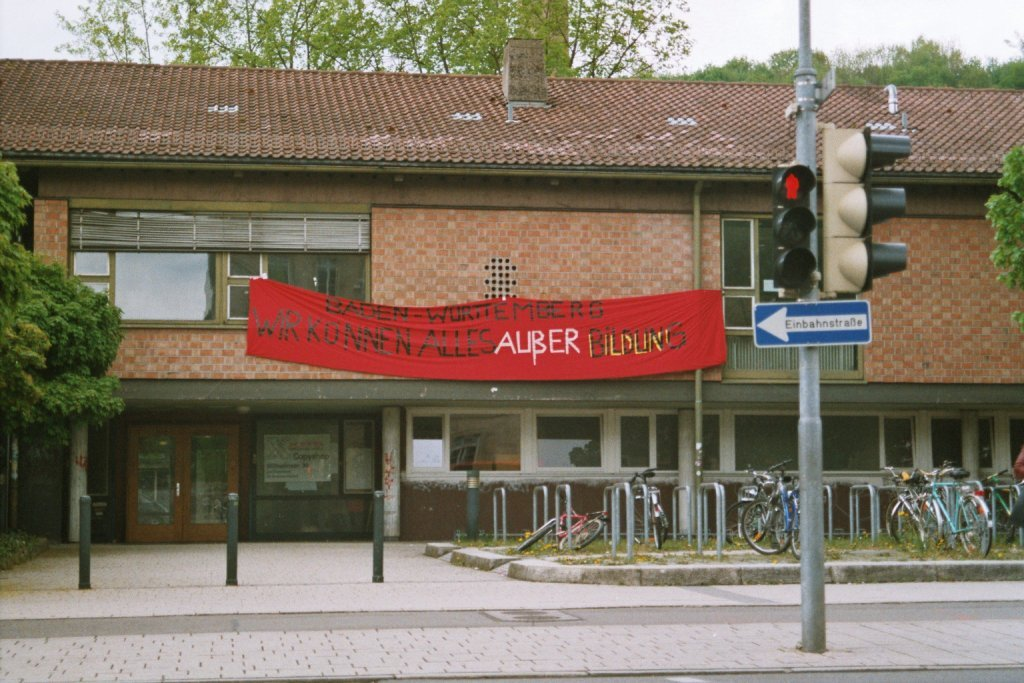
\includegraphics[width=\linewidth]{pictures/clubhaus.jpg} \\
				\footnotesize http://mapio.net/o/2026708/
			\end{column}
		\end{columns}
	\end{frame}
\begin{frame}
	\center{\Huge{24.10}}\\
	\center{CHF der Fachschaft Info, Kogni und Psycho}
	
\end{frame}


		\begin{frame}{u.v.a.m.}
			\centering 
			\begin{huge}
				Und noch viel mehr anderen geilen Scheiß!
			\end{huge}
			\vspace*{0.5cm}\\
			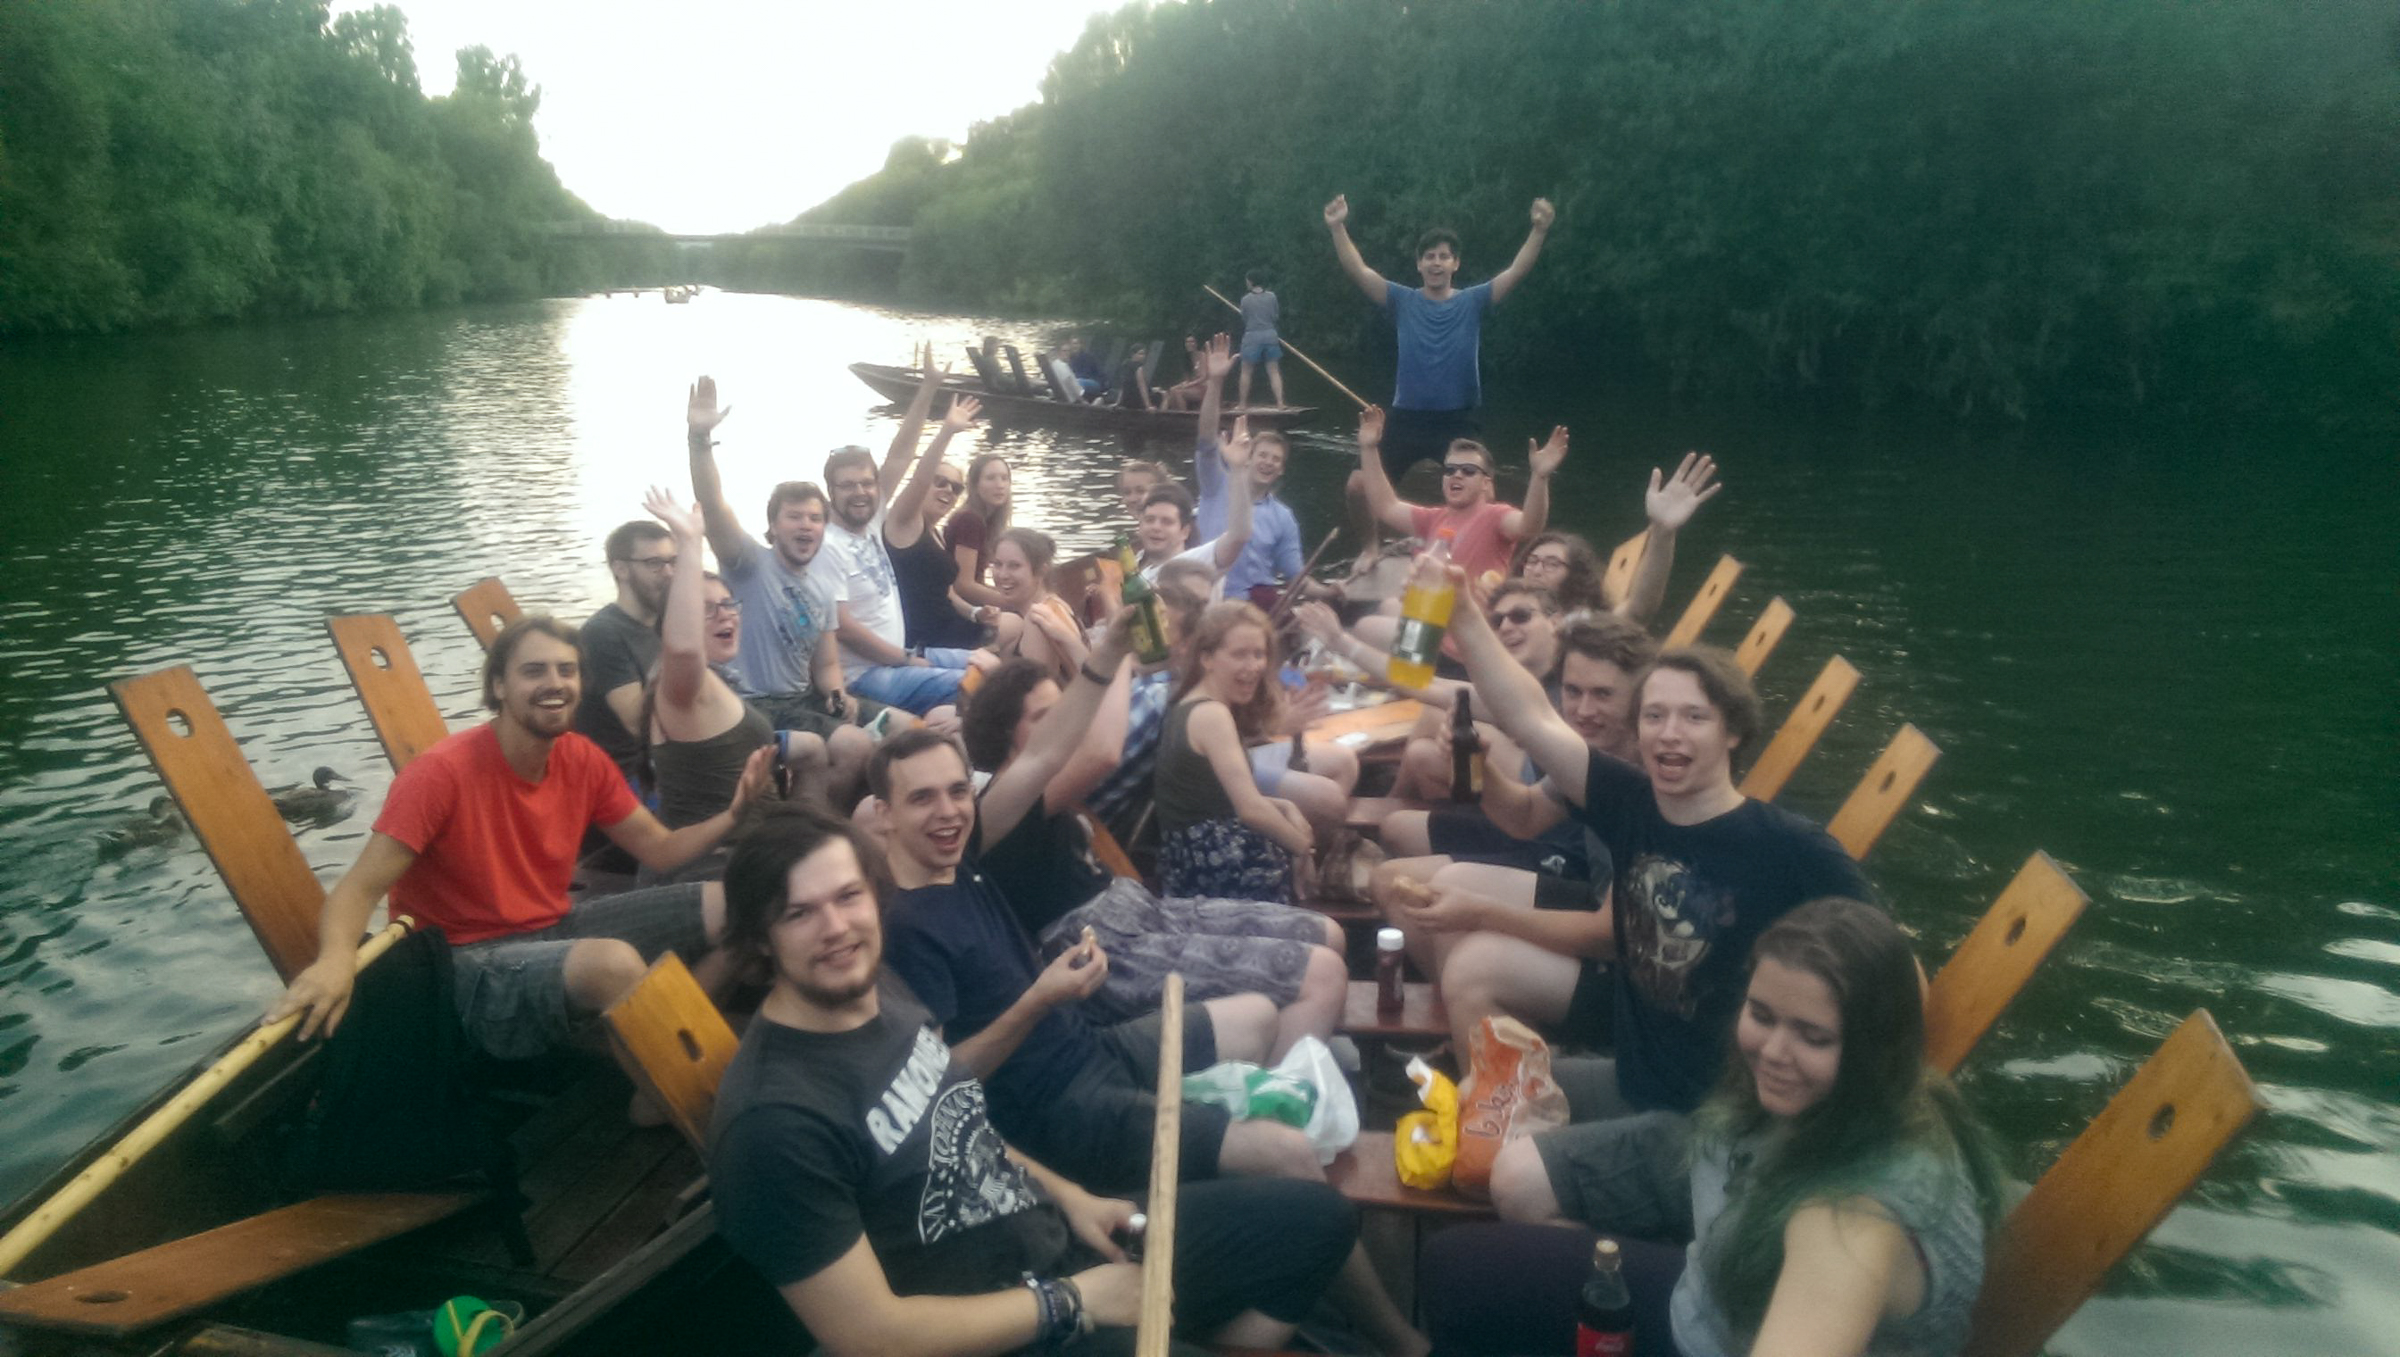
\includegraphics[height=0.6\textheight]{pictures/stocherkahn.jpg}
		\end{frame}
	
	\begin{frame}{Fachschaftsarbeit}
		\framesubtitle{wie geht das?}
		\pause 
		\begin{columns}
			\begin{column}{.5\linewidth}
				\begin{itemize}[<+->]
					\item einfach vorbeikommen und mitmachen ;-)
					\item regelmäßige Treffen im Fachschaftszimmer (Sand, Zimmer C125)
					\item nächstes Treffen: \\Donnerstag 31.10.19 18:30 Uhr
					\item teilweise weitere Treffen zu Teilbereichen der Fachschaftsarbeit
					\item Kogni-Treffen: 31.10.19 18:00 Uhr
					\item \textbf{Kommt vorbei!}
				\end{itemize}
			\end{column}
			\begin{column}{0.5\linewidth}
				\includegraphics[width=0.7\linewidth]{pictures/uebersicht_sand.pdf}\\
				\includegraphics[width=0.7\linewidth]{pictures/uebersicht_pi.pdf}\\
			\end{column}
		\end{columns}
	\end{frame}
	
%	\begin{frame}{Freizeit}
%		\centering 
%		
%	\end{frame}
	
	\begin{frame}
		\begin{columns} 
			\column{0.3\textwidth}
			\includegraphics[width=\linewidth]{pictures/keepcalm.pdf}
			\column{0.3\textwidth}
			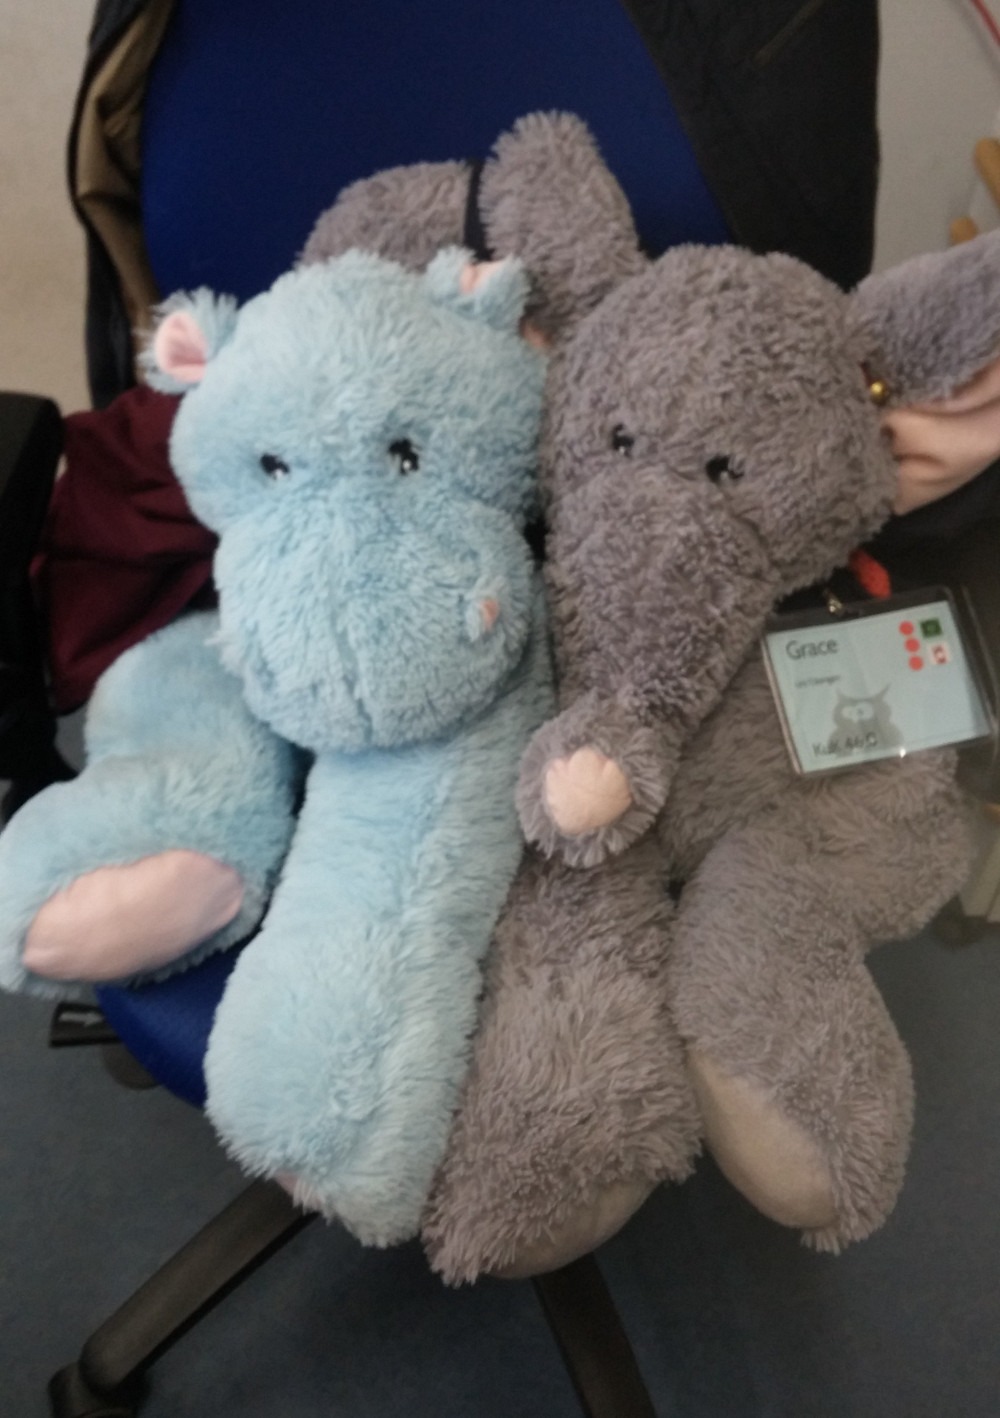
\includegraphics[width=0.9\linewidth]{pictures/grace_siggi.jpg}
			\column{0.4\textwidth}
			\centering
			\begin{huge}
				Wir freuen uns auf euch! \vspace*{1cm}
			\end{huge}
			
			\qrcode{https://www.fsi.uni-tuebingen.de}\\
			\begin{scriptsize}
				\url{https://www.fsi.uni-tuebingen.de}\\
				\url{http://fsi-tue.de}
			\end{scriptsize}
		\end{columns}
		
	\end{frame}

\end{document}
